\section{Introduction}
%Large language models (LLMs) \citep{brown2020language,touvron2023llama,dubey2024llama} have demonstrated remarkable capabilities, including text comprehension \citep{devlin2018bert}, generation \citep{radford2019language,goyal2020evaluating,roziere2023code}, and reasoning \citep{raffel2020exploring,wei2022chain}. A significant proportion of LLMs research focuses on external behaviors, such as task-based evaluations \citep{srivastava2022beyond,bubeck2023sparks} and designing prompts to enhance performance \citep{liu2021generated,wang2022self}. However, the inner mechanisms of LLMs remain largely unexplored, with ongoing concerns about the validity of their interpretability \citep{ghorbani2019interpretation,wen2024transformers}, and the theoretical understanding of transformers \citep{vaswani2017attention}, the core components of LLMs, is still limited.

Recent analyses of transformer-based open-source large language models (LLMs), such as GPT-2 \citep{radford2019language}, Llama-2 \citep{touvron2023llama}, Llama-3 \citep{dubey2024llama}, Mixtral \citep{jiang2023mistral}, and Pythia \citep{biderman2023pythia}, have revealed three intriguing phenomena: 
\begin{itemize}[leftmargin=2em]
\setlength\itemsep{-0.3em}
\item[-] \textbf{Attention sinks} \citep{xiao2023efficient}: In many attention heads, the initial token consistently attracts a large portion of the attention weights. Other special tokens, such as the delimiter token, can also draw significant attention weights. These tokens are collectively referred to as \emph{sink tokens}. 
\item[-] \textbf{Value-state drains} \citep{guo2024attention}: For the attention heads that exhibit attention sinks, the value states of sink tokens are consistently much smaller than those of other tokens. 
\item[-] \textbf{Residual-state peaks} \citep{sun2024massive}: The residual states of sink tokens, excluding those from the first and last layers, exhibit significantly larger norms compared to other tokens. 
% \item[-] \textbf{Attention-logit concentration}: We further find that The attention logits corresponding to the key of the sink token and queries of all non-sink tokens are nearly identical. 
% The attention logits corresponding to the key of the sink token and queries of all non-sink tokens are nearly identical. 
\end{itemize}
These phenomena often appear together and consistently occur in various pretrained LLMs, which we collectively refer to as the \emph{extreme-token phenomena}. Figure \ref{figure:extreme-token} illustrates these phenomena in Llama-3.1-8B-Base, using a fixed prompt sentence: “\bos Summer is warm\period~Winter is cold\period”. Here, the first token, \bos~(the Beginning-of-Sequence token), serves as the sink token. As shown in the figure, the sink token receives disproportionately high attention weights, exhibits significantly smaller value states, and has much larger residual state norms compared to other tokens. It is important to note that the first token does not have to be \bos~to act as a sink token; other tokens appearing first in the sequence can also serve this role. Additionally, in models such as Llama-2, a delimiter token can also function as the sink token. 

\begin{figure}[t]
  \centering
  \begin{subfigure}[t]{0.32\textwidth}
      \centering 
      \caption{\small Attention weights at L24}
      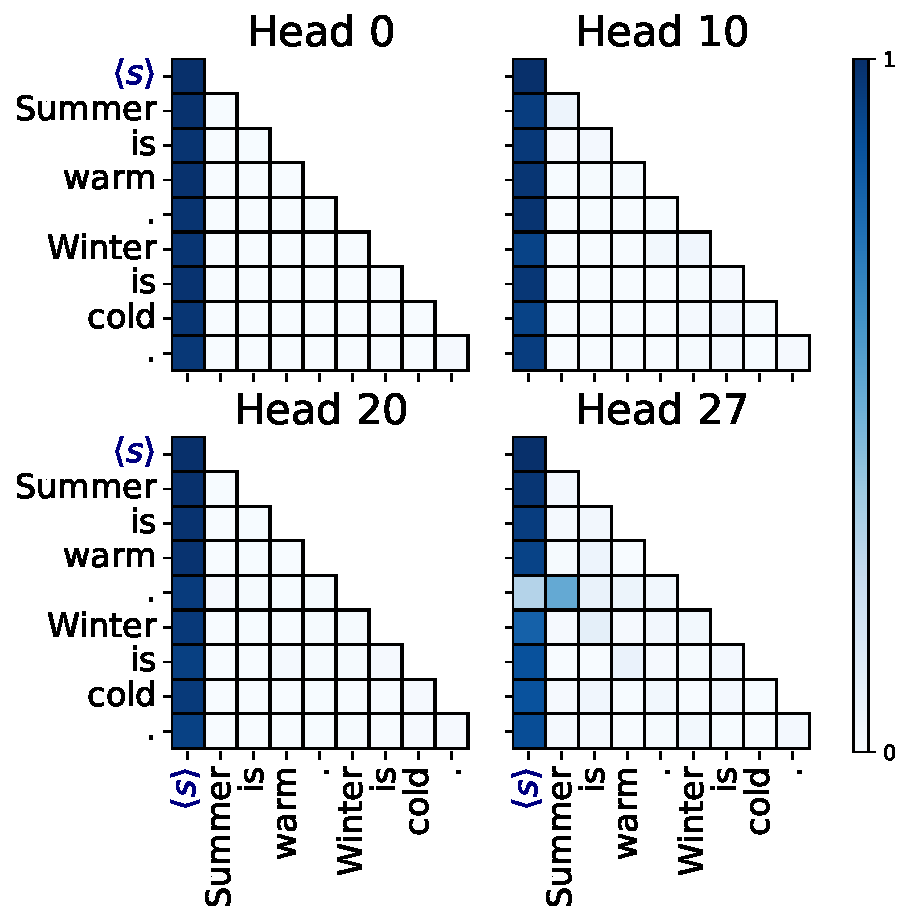
\includegraphics[width=0.9\textwidth]{Figures/demo_attn_sink.pdf}
      \label{fig:attention_sinks_wide_random}
  \end{subfigure}
  \hfill
  % \begin{subfigure}[t]{0.32\textwidth}
  %     \centering 
  %     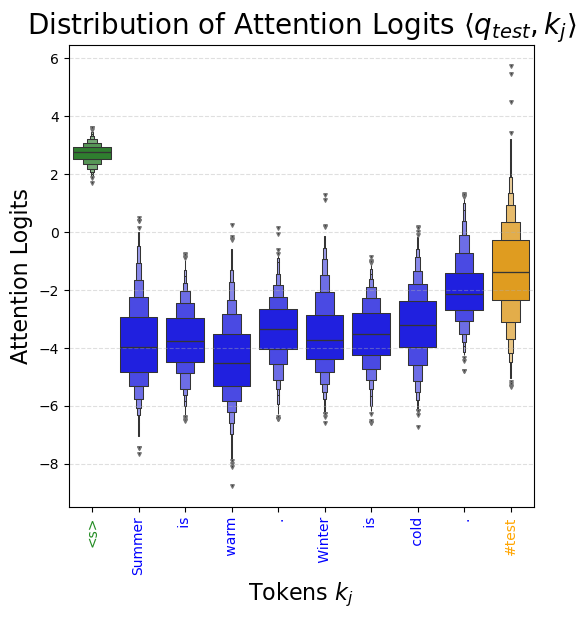
\includegraphics[width=\textwidth]{Figures/attn_logits_random_tokens.png}
  %     \caption{\small Attention logits \(\langle \bm{q}_{\mathrm{test}}, \bm{k}_{j}\rangle\).}
  %     \label{fig:attention_logits_random}
  % \end{subfigure}
  \begin{subfigure}[t]{0.3\textwidth}
      \centering 
      \caption{\small Norms of value states}
      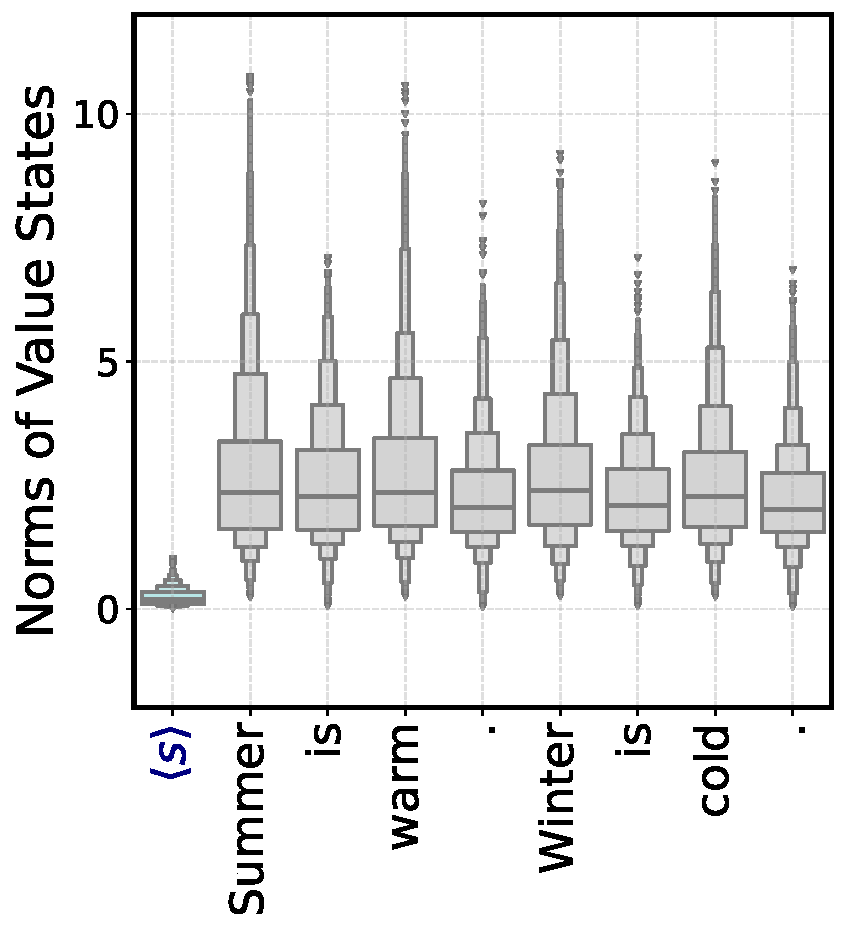
\includegraphics[width=0.9\textwidth]{Figures/demo_val_drain.pdf}
      \label{fig:value_norms_zeroed}
  \end{subfigure}
  \hfill
  \begin{subfigure}[t]{0.3\textwidth}
      \centering 
      \caption{\small Norms of residual states}
      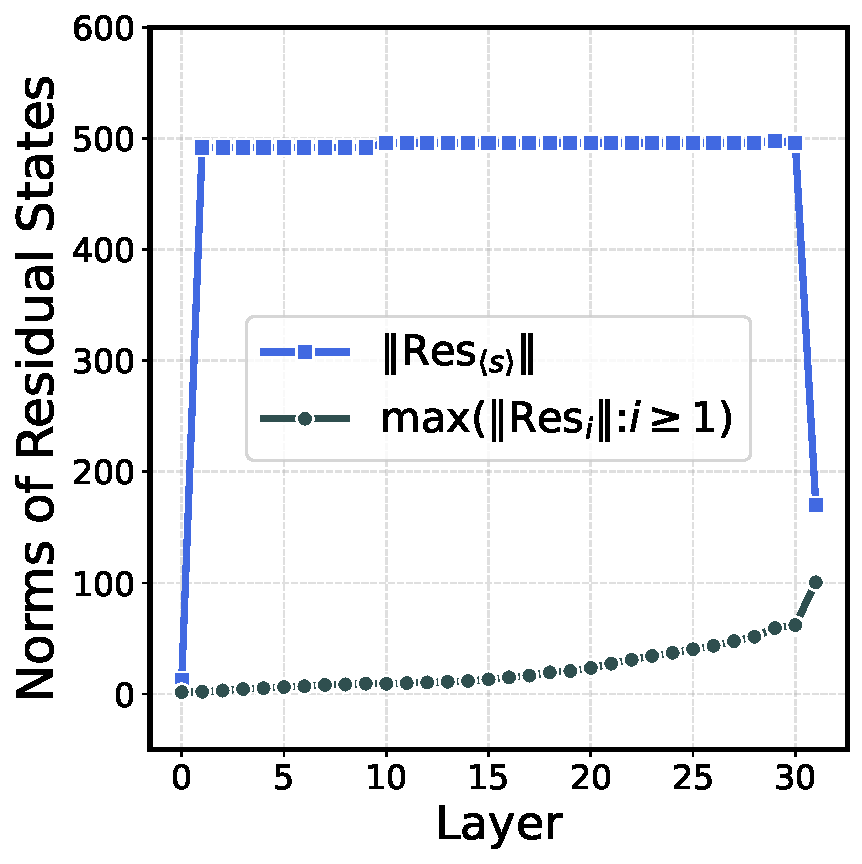
\includegraphics[width=0.9\textwidth]{Figures/demo_res_peak.pdf}
      \label{fig:token_norms_massive}
  \end{subfigure}
  
  % \begin{minipage}{0.33\textwidth}
  %     \centering
  %     \subcaption{\small Attention logits}
  %     \label{fig:circuit-attn-logits}
  %     \vspace{-.2em}
  %     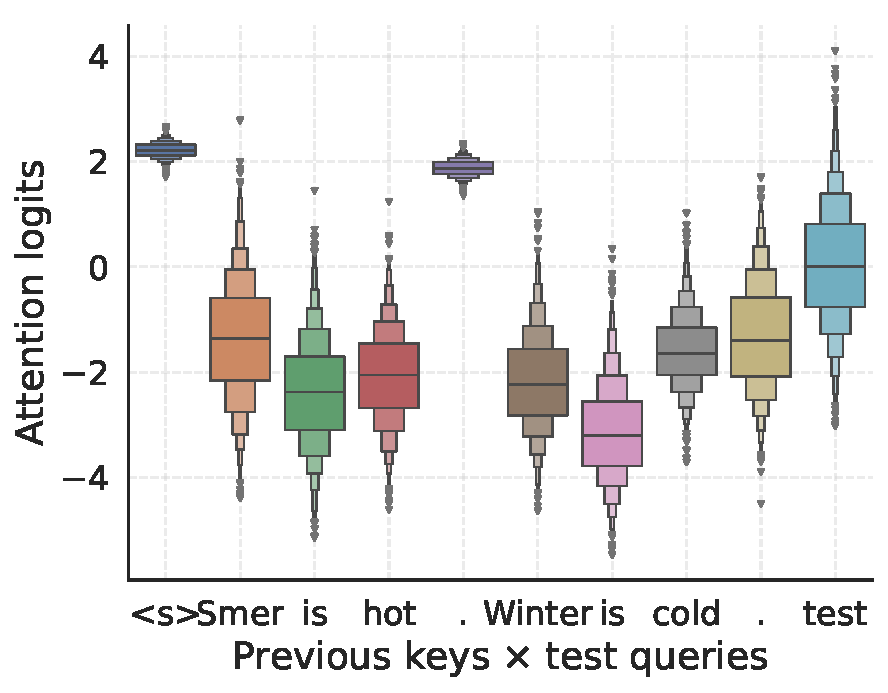
\includegraphics[width=\linewidth]{Figures/figures_circuit/logits.pdf}
  % \end{minipage}~
  % % \hspace{-1em}
  % \begin{minipage}{0.33\textwidth}
  %     \centering
  %     \subcaption{\small Residual states norm}
  %     \label{fig:circuit-massive-norm}
  %     \vspace{-.2em}
  %     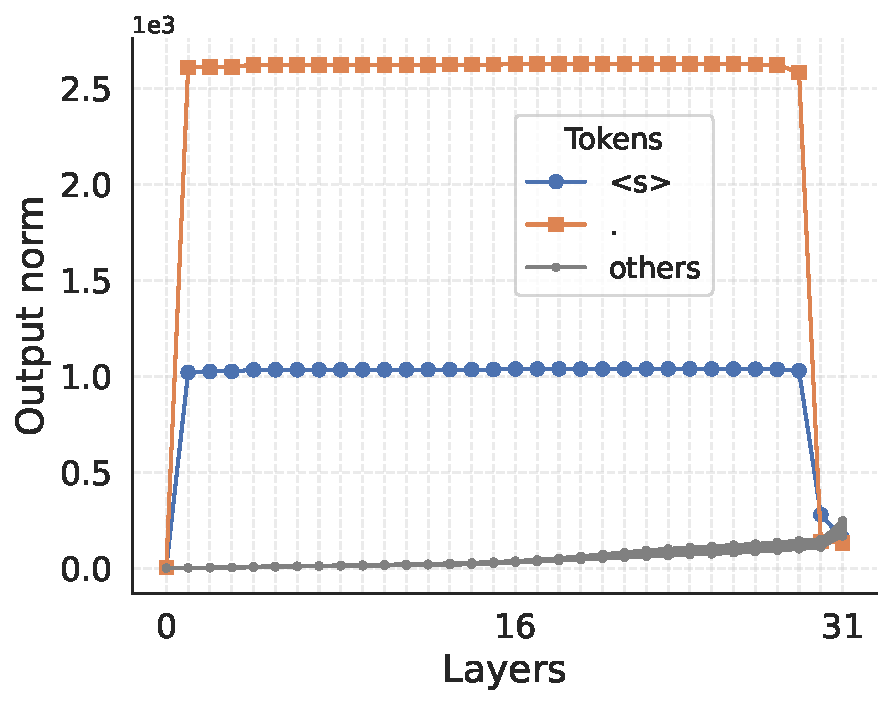
\includegraphics[width=\linewidth]{Figures/figures_circuit/massive.pdf}
  % \end{minipage}
  % \hspace{-1em}
  % \begin{minipage}{0.33\textwidth}
  %     \centering
  %     \subcaption{\small Value states norm}
  %     \label{fig:circuit-value-norm}
  %     \vspace{-.2em}
  %     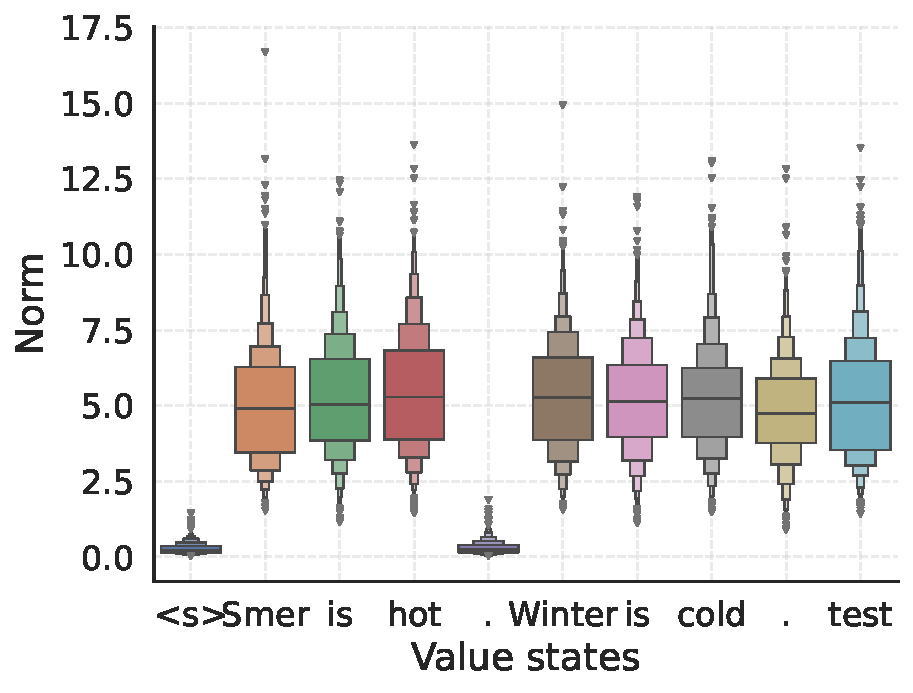
\includegraphics[width=\linewidth]{Figures/figures_circuit/values.pdf}
  % \end{minipage}
  \vspace{-0.5em}
  \caption{\small \textbf{Extreme-token phenomena in Llama 3.1.}
  %\tianyu{bigger text size; remove all labels in the middle of fig (a); notations; thicker lines;  remove all test tokens. backup plan: include more heads} 
  We evaluate the attention weights, value states norm, and residual states norm on the Llama 3.1-8B-Base model, where the input sentence is ``\bos Summer is warm\period~Winter is cold\period''.  \textit{Left (a)}: The attention weights across multiple heads at Layer 24. We observe the \textit{attention sink} phenomenon: the \bos{} token attracts a significant portion of the overall attention weight.
 % Figure \ref{fig:attention_logits_random} displays the distribution of attention logits \(\langle \bm{q}_{\mathrm{test}}, \bm{k}_{i}\rangle\) across all heads and test tokens at Layer 24. %\sm{which head?}. 
  %The logits for the \bos~token 
  %~and the first \delim~
  %are concentrated at large values, while those for other tokens are smaller and fluctuate across different random test tokens. 
  \textit{Middle (b)}: The empirical distribution of the norms of value states over all layers 
  %\sm{all or 1-30?} \DP{all}
  and all heads. We exclude 2\% of the outlier values to help visualization. We observe the \textit{value-state drain} phenomenon: the value state of the \bos~token is much smaller than those of other tokens on average.
  \textit{Right (c)}: The norm of the residual stream states, measured at the output of each layer. We observe the \textit{residual-state peak} phenomenon: the \bos~token's residual states have significantly larger norms than those of other tokens from layers 1 to 30. We present the extreme-token phenomena over other input sequences in Appendix~\ref{sec:many_samples}.
  %\tianyu{add links to appendix} %\sm{Truncate y axis of (b) at 12. }
  }
  \label{figure:extreme-token}
  \vspace{-1em}
\end{figure}

The extreme-token phenomena have posed several challenges for pretrained transformers in downstream tasks. For instance, sink tokens require special treatment during long-context inference \citep{xiao2023efficient, han2023lm, yu2024unveiling, chen2024image} and model quantization \citep{dettmers2022gpt3, liu2024intactkv, son2024prefixing} to maintain high levels of performance. Additionally, attention sinks have reduced the interpretability of attention maps in vision transformers \citep{darcet2023vision}. To address these issues, \citet{sun2024massive} and \citet{darcet2023vision} propose adding a ``special token'' to transformers to serve as the sink token, preventing other tokens from becoming sinks. However, even this special token still exhibits extreme-token phenomena. Despite these efforts, no prior work has satisfiably explained the mechanisms behind the extreme-token phenomena. \citet{xiao2023efficient} proposes a hypothesis for why they occur, suggesting that models tend to dump unnecessary attention values to specific tokens. 

% \sm{I am here}

This work aims to demystify the extreme-token phenomena in LLMs. We demonstrate that these phenomena arise from an \textit{active-dormant mechanism} in attention heads (cf.\ Claim~\ref{claim:active-dormant}), coupled with a \textit{mutual-reinforcement mechanism} during pretraining (cf.\ Claim~\ref{claim:mutual-reinforcement}). We support these statements through studies on simplified transformer architectures and tasks, a dynamical theory for these models, and experiments on pretrained LLMs. The structure of the paper and our key contributions are outlined as follows:
\begin{enumerate}[leftmargin=2em]
\setlength\itemsep{0pt}
\item In \Cref{sec:bb_task},  we train one- to three-layer transformers on a simple task called the \textit{Bigram-Backcopy} (BB) task, which also displays extreme-token phenomena similar to those observed in LLMs. We show that attention sinks and value-state drains are a consequence of the \textit{\activedormant} (cf.\ Claim~\ref{claim:active-dormant}). Both theoretically and empirically, we demonstrate that \textit{mutual reinforcement mechanism} (cf.\ Claim~\ref{claim:mutual-reinforcement}) dynamically drives these phenomena: attention sinks and value-state drains reinforce one another, leading to a stable phase where all query tokens generate near identical attention logits for the keys of extreme tokens. Additionally, empirical results reveal that residual-state peaks arise from the interaction between this mutual reinforcement mechanism and the Adam optimization algorithm. 
\item In \Cref{sec:llm}, we demonstrate the \textit{\activedormant}~in pre-trained LLMs by showing that many attention heads transition between active and dormant phases based on the input domain. Specifically, we identify an interpretable active-dormant head (Layer 16, Head 25 in Llama 2-7B-Base \citep{touvron2023llama}) that activates on GitHub data but remains dormant on Wikipedia data. Moreover, in examining the dynamics of OLMo-7B-0424 \citep{groeneveld2024olmo}, we observe the same mutual reinforcement mechanism and stable phase, consistent with those found in the BB task. This demonstrates that the simple BB model captures both the static and dynamic properties of extreme-token phenomena in LLMs and accurately predicts their behavior. 
 % We also discover circuits in LLMs related to extreme tokens that partially align with models trained on the BB task. 
 % Specifically, the logits corresponding to the key of the extreme token and queries of all non-extreme tokens ($ \text{logit}_{\bos}$), 
\item Importantly, the quantitative properties of extreme-token dynamics show strong consistency among the theoretical and empirical results of the Bigram-Backcopy task and the empirical performance of OLMo. In particular, we consistently observe the \textbf{sink-logits concentration} phenomenon, where the logits corresponding to the key of the extreme token and the queries of all non-extreme tokens ($ \text{logit}_{\cdot,\bos}$) are nearly identical—an observation not previously documented in the literature. We summarize the aligned results between the theoretical and empirical findings of the Bigram-Backcopy task and the empirical performance of LLMs in Table~\ref{tab:consistent_transposed}. 

 % Specifically, the BB task demonstrate logarithmic growth of the difference of attention logits on the extreme token and the average of attention logits on other tokens ($\Delta \text{logit}_{\text{Extreme}}$), the monotonic decrease of the value state norm of the extreme token ($\|\vall_{\text{Extreme}}\|$), and the linear growth of the norm of the residual state $\|\res_{\text{Extreme}}\|$.  %\tianyu{I tried to write a description, but it's too long, so I decide to only keep this and commented out some drafts}
% \begin{table}[h]
%     \centering
%     \caption{Consistent results across theory, Bigram-Backcopy task, and LLMs. The \checkmark~denotes consistent results, and the $\star$ denotes partial match. \tianyu{I should polish this table later.. I'm not sure how to lay out the results, though.}}
%     \label{tab:consistent}
%     \begin{tabular}{c|cccc}
%     \toprule
%          &  \makecell{$\text{logit}_\bos$\\
%          $\log$-growth } & \makecell{$\|\vall_\bos\|$\\monotonic decrease} &  \makecell{$\|\res_\bos\|$\\linear growth} & \makecell{$\text{logit}_\bos$\\
%          concentration }\\
%        \midrule
%        Theory  &  \checkmark & \checkmark & $\star$ & \checkmark \\
%        BB-task & \checkmark   & \checkmark & \checkmark & \checkmark\\
%        LLMs & $\star$  & \checkmark & \checkmark & \checkmark\\
%     \bottomrule
%     \end{tabular}
% \end{table}
\item We propose architectural and optimization modifications to mitigate the extreme-token phenomena. Specifically, we demonstrate that replacing SoftMax with ReLU activations in attention heads eliminates extreme-token phenomena in the BB task, while switching from Adam to SGD removes the residual-state peak phenomenon. We discuss the possibility that similar modifications could mitigate extreme-token phenomena in LLMs. %\sm{Figure for active-dormant. Figure for mutual-reinforcement. } \tianyu{find algorithm selection in TF as statistician}%\tianyu{I still feel that this looks not so strong.} %\DP{The phrasing should be like: We conclusively demonstrate that the extreme-token phenomenon is a property of the specific architecture and optimization procedure, and show this via two ablation tests in the BB task: replacing SoftMax with ReLU in the attention mechanism and switching Adam to SGD. Our work demonstrates potential classes of mechanisms to mitigate extreme-token phenomena in LLMs.}
\end{enumerate}

\begin{table}
    \centering
    \begin{tabular}{|c|c|c|c|}
    \hline
         & BB-task Theory & BB-task Experiments & LLM Experiments \\
    \hline
    \makecell{$\Delta \text{logit}_{\cdot,\bos}$ $\log$-growth} & \checkmark & \checkmark & $\star$ \\ \hline
    \makecell{$\|\vall_{\bos}\|$ monotonic decrease} & \checkmark & \checkmark & \checkmark \\ \hline
    \makecell{$\|\res_{\bos}\|$ linear growth} & $\star$ & \checkmark & \checkmark \\ \hline
    \makecell{$\text{logit}_{\cdot,\bos}$ concentration} & \checkmark & \checkmark & \checkmark \\
    \hline
    \end{tabular}
        \caption{Consistency of the quantitative properties across the theoretical and empirical results of the Bigram-Backcopy task and empirical results of LLMs. A \checkmark~denotes a consistent result, while a $\star$ denotes an inconclusive result. The $\text{logit}_{\cdot,\bos}$ denotes logits corresponding to the key of the extreme token and queries of all non-extreme tokens, i.e., the $\query_{\cdot}^\top \key_{\bos}$. The $\Delta \text{logit}_{\cdot,\bos}=\text{logit}_{\cdot,\bos}-\text{Mean}[\text{logit}_{\cdot,\text{others}}]$ is a progress measure for attention sinks. The $\|\vall_{\bos}\|$ denotes the value state norm of the extreme token, and $\|\res_{\bos}\|$ denotes the residual state norm of the extreme token. See \Cref{sec:prelim_notation} for the definitions of these notations. }
    \label{tab:consistent_transposed}
\end{table}


% \begin{enumerate}[leftmargin=2em]
% \setlength\itemsep{0pt}
% \item We design the \textit{Bigram-Backcopy} (BB) task, train one-to-three layer transformers, and recapitulate the extreme token phenomena, offering a framework for understanding the \activedormant. Both theoretically and empirically, we demonstrate the mutual reinforcement dynamics of the extreme token phenomena. Our key finding is that the attention sinks and value-state drains reinforce each other in the dynamics, leading to the stable phase consists of identical attention logits from all query tokens to the key of extreme tokens. With empirical evidence, we demonstrate that residual-state peaks result from the interaction of this mutual reinforcement mechanism with Adam.
% \item Extending the findings from small models to LLMs, we first discover an interpretable active-dormant head (Layer 16 Head 25 in Llama 2-7B-Base \citep{touvron2023llama}), verified through causal interventions. We also discover circuits in LLMs for the extreme tokens that partially match the models trained for the BB task. We inspect the dynamics of OLMo-7B-0424 \citep{groeneveld2024olmo}, identifying the same mutual reinforcement mechanism and stable phase, consistent with predictions from the BB task analysis.
% \item As broader implications, we demonstrate potential design choices to mitigate extreme-token phenomena in LLMs. we propose two methods to eliminate the extreme-token phenomena based on the discovered mechanisms: replacing SoftMax with ReLU activations in attention heads and switching Adam to SGD, both verified in the BB task. \tianyu{I still feel that this looks not so strong.} \DP{The phrasing should be like: We conclusively demonstrate that the extreme-token phenomenon is a property of the specific architecture and optimization procedure, and show this via two ablation tests in the BB task: replacing SoftMax with ReLU in the attention mechanism and switching Adam to SGD. Our work demonstrates potential classes of mechanisms to mitigate extreme-token phenomena in LLMs.}
% \end{enumerate}






% \yub{LLMs...}~\yub{a sophisticated but extremely powerful system}~\yub{however are there any structural biases?}

% \yub{some recent works identify an intruiging phenomenon in trained LLMs.}~\yub{describe the sink token phenomenon.}~\yub{two features: massive in norm, and caused by massive in specific entries~\citep{sun2024massive}, and attract attention scores (give rigorous description)~\citep{xiao2023efficient,darcet2023vision}}~\yub{Has been used in applications such as Streaming LLM generation~\citep{xiao2023efficient,han2023lm}.}

% Despite the intriguing findings, the understanding is still~\yub{at a surface level}, with many questions unanswered.~\yub{1. what tokens get to be sink tokens, and how is this process related to the position of the tokens in the sequence?}~\yub{second delimiter thing...}~\yub{2. is attention concentration phenomenon a consequence of the massive norms?}~\yub{3. Does attention concentration imply that non-sink tokens are not important to the final attention output?}


% In this work, we provide a more in-depth understanding on how sink tokens arise and take effect in trained LLMs. Our contributions can be summarized as follows.
% \begin{itemize}
%     \item BLAH.
% \end{itemize}



%!TEX root = ../main.tex

\section{Related Work}
\label{sec:related}

\textbf{State space models} have shown promise in modeling sequential data, including time series data~\citep{gu2022efficiently}, audio~\citep{goel2022s}, and visual data~\citep{nguyen2022s4nd}.
Our model builds off work on simplifying and parameterizing diagonal versions of S4~\citep{gu2022parameterization,gupta2022diagonal, gu2022train}.
Gated state spaces~\citep{mehta2022long} also aim to adapt SSMs to language modeling, but our results suggest that the GSS model does not perform as well as \hthree (or even as well as earlier SSMs like S4D).
The idea to combine SSMs with attention in hybrid models is not new; Mehta et al.~\citep{mehta2022long} also showed that interleaving attention with their GSS layer can improve performance, which we also validate on our OpenWebText experiments.
These positive results suggest that attention and SSMs are complementary, and that hybrid models may be a promising direction for future work.

\textbf{Large language foundation models}~\citep{bommasani2021opportunities} have demonstrated the power of scaling attention-based networks to billions of parameters and training them on trillions of tokens~\citep{hoffmann2022training}.
Understanding the mechanistic basis~\citep{elhage2021mathematical} behind these models may yield insights into better design choices for future models.
These and similar explorations have informed the design of \hthree and our selection of synthetic languages.
A number of recent works have also explored how to address the shortcomings of attention by approximating the attention computation~\citep{wang2020linformer,katharopoulos2020transformers, choromanski2020rethinking,tay2020long, kitaev2020reformer, daras2020smyrf}.
We believe these efforts are complementary to SSMs, and we are excited to see how they can be combined in future work.

\textbf{Linear attention}~\citep{katharopoulos2020transformers} and classical sequence models like RNNs serve as inspiration for \hthree.
Appendix~\ref{app:linear_attention} draws a direct connection between linear attention and LTI systems.
Luo et al.~\citep{luo2021stable} also propose a variant of linear attention that can achieve $O(n \log n)$ scaling in sequence length.
Appendix~\ref{sec:app_additional_experiments} evaluates linear attention on language modeling, and finds that it underperforms exact attention, whereas \hthree outperforms attention.
The multiplicative interactions in \hthree are reminiscent of gating mechanisms in LSTMs~\citep{hochreiter1996lstm} and GRUs~\citep{cho2014properties}, which suggests that architectural lessons from these sequence models may be useful for adapting SSMs to language modeling.
A number of algorithms for scaling attention to longer sequences have also been proposed, such as Transformer-XL~\citep{dai2019transformer}, Reformer~\citep{kitaev2020reformer}, Performer~\citep{choromanski2020rethinking}, and Perceiver AR~\citep{hawthorne2022general}.
Some of these approaches underperform exact attention on language modeling, and may be slower in wall-clock speed~\citep{dao2022flashattention}.
A thorough comparison of these alternatives to exact attention and how well they scale in model size and amount of training data is fruitful future work.

\textbf{FFT} algorithms are used in a wide variety of applications, including signal processing~\citep{oppenheim1978applications}, control theory~\citep{brogan1974modern}, and more.
Various algorithms for computing the FFT have existed for decades~\citep{oppenheim2001discrete}.
We hope our work on appealing to these classic algorithms to accelerate new applications such as learned SSMs will inspire future algorithmic exploration, even if hardware is not designed for them~\citep{hooker2021hardware}.

%%% Local Variables:
%%% mode: latex
%%% TeX-master: "../main"
%%% End:


\subsection{Preliminaries and notations}\label{sec:prelim_notation}

% Throughout this paper, we let $\sigma(t)\defeq \relu(t)=\max\sets{t,0}$ denote the standard relu activation. 
 % 

While different LLMs may use slightly varying transformer architectures, most use the structure proposed by \cite{vaswani2017attention}, with the key modification being the shift from post-norm to pre-norm. We represent the tokenized input sequence of length $n$, with positional embeddings included, as $\bH = [\bh_1, \dots, \bh_n]\in \R^{d \times n}$, where $\bh_i$ denotes the $i$th input token, and $d$ is the embedding dimension. We denote the layer-normalization operation as $\LN$, the column-wise SoftMax operation as $\softmax$, the causal-mask as $\mask$, and the pointwise ReLU function as $\relu$. 

The transformer architecture applies causal-attention and MLP layers iteratively to the input sequence $\bH$. A causal-attention layer with $M$ heads is represented as $\Attn(\cdot)$, parameterized by $\sets{ (\bQ_m,\bK_m, \bV_m, \bO_m)}_{m}$: 
\begin{talign}
\label{eqn:attention}
\Attn(\bH) \defeq \sum_{m = 0}^{M-1}  \attn_{m}(\bH)\in \R^{d \times n},
\end{talign}
where each attention head $\attn_m(\cdot)$ is given by
\begin{talign}\label{eqn:attention_head_prelim}
\attn_m(\bH) \defeq  \bO_m \bV_m \LN(\bH) \softmax\paren{\mask\paren{ \LN(\bH)^\top \bK_m^\top \bQ_m \LN(\bH) }}. 
\end{talign}
We denote the attention map as ${\sf Map}=\softmax\paren{\mask\paren{ \LN(\bH)^\top \bK_m^\top \bQ_m \LN(\bH) }}$, and typically plot its transpose, ${\sf Map}^\top$, in figures.

An MLP layer, denoted $\mlp(\cdot)$, has parameters $(\bW_1,\bW_2)$:
\begin{talign}\label{eqn:MLP_layer_prelim}
\mlp(\bH) \defeq \bW_2 \relu(\bW_1 \LN(\bH) ) \in \R^{d \times n}.
\end{talign}
An $L$-layer transformer consists of a composition of $L$ self-attention and MLP layers with residual connection structure. Given an input $\bH^{(0)} \in \R^{d \times n}$, the output of the $L$-layer transformer, $\bH^{(L)}$, is computed as follows: 
\begin{talign}
\bH^{(\ell + 1)} =\bH^{(\ell + 1/2)} +  \mlp^{(\ell)}\paren{ \bH^{(\ell + 1/2)}},~~~ \bH^{(\ell + 1/2)} = \bH^{(\ell)} + \Attn^{(\ell)}\paren{\bH^{(\ell)}},~~~ \ell\in\set{0,\dots,L-1}.
\end{talign}
For consistency between the code and the text, we adopt zero-indexing throughout this paper, meaning that attention head and layer indices begin at $0$ instead of $1$. 

For the output $\bH^{(\ell + 1)}$ of layer $\ell$, we define the residual state $\res_{\tok}$ of a token $\tok \in \{0, 1, \ldots, n-1\}$ as the $\tok$th column of $\bH^{(\ell + 1)}$. For a specific layer $\ell$ with input $\bH^{(\ell)} \in \R^{d \times n}$, and for a specific attention head $m$ with query, key, and value matrices $(\bQ, \bK, \bV, \bO)$, we define the \textit{query}, \textit{key}, and \textit{value states} $(\query_\tok, \key_\tok, \val_\tok)$ of a token $\tok \in [n]$ as the $\tok$th columns of $\bQ \bH^{(\ell)}$, $\bK \bH^{(\ell)}$, and $\bO \bV \bH^{(\ell)}$, respectively\footnote{We define the value state as $\bO \bV \bH$ rather than $\bV \bH$ since what is added to the residual state is essentially $\bO \bV \bH$. }. The \textit{attention logit} $\text{logit}_{\tok^\prime, \tok}$ is defined as the $(\tok^\prime, \tok)$th element of $(\bH^{(\ell)})^\top \bQ^\top \bK \bH^{(\ell)}$. For notation simplicity, we omit the dependence on $\ell$ and $m$ in $(\query_\tok, \key_\tok, \val_\tok, \text{logit}_{\tok^\prime, \tok})$, as these will be clear from context.  Additionally, for a fixed token $\tok$, we use the shorthand $\text{logit}_{\cdot,\tok}$ for the set $\{\text{logit}_{\tok^\prime, \tok} \mid \tok^\prime\in\vocab\}$.

% Here, we introduce the notations and the transformer architecture. While different LLMs may use slightly varying transformer architectures, most use the structure proposed by \cite{vaswani2017attention}, with the key modification being the shift from post-norm to pre-norm. We represent the tokenized input sequence of length $n$, with positional embeddings included, as $\bH=[\bh_1; \dots; \bh_n]\in \R^{n \times d}$, where $\bh_i$ denotes the $i$th input token, and $D$ is the embedding dimension. We denote the layer-normalization operation as $\LN$, the row-wise SoftMax operation as $\softmax$, the causal-mask as $\mask$, and the pointwise ReLU function as $\relu$. 

% The transformer architecture applies causal-attention and MLP layers iteratively to the input sequence $\bH$. A causal-attention layer with $M$ heads is represented as $\Attn(\cdot)$, parameterized by $\sets{ (\bQ_m,\bK_m, \bV_m, \bO_m)}_{m}$: 
% \begin{talign}
% \label{eqn:attention}
% \Attn(\bH) \defeq \bH + \sum_{m = 0}^{M-1} \attn_{m}(\bH) \bO_m \in \R^{n \times D},
% \end{talign}
% where each attention head $\attn_m(\cdot)$ is given by
% \begin{talign}\label{eqn:attention_head_prelim}
% \attn_m(\bH) \defeq \softmax\paren{\mask\paren{ \LN(\bH) \bQ_m \bK_m^\top \LN(\bH)^\top }} \cdot \LN(\bH) \bV_m. 
% \end{talign}
% An MLP layer, denoted $\mlp(\cdot)$, has parameters $(\bW_1,\bW_2)$:
% \begin{talign}\label{eqn:MLP_layer_prelim}
% \mlp(\bH) \defeq \bH + \relu(\LN(\bH) \bW_1) \bW_2 \in \R^{n \times D}.
% \end{talign}
% An $L$-layer transformer consists of a composition of $L$ self-attention layers, each followed by an MLP layer. Given an input $\bH^{(0)} \in \R^{n \times D}$, the output of the $L$-layer transformer, $\bH^{(L)}$, is computed as follows: 
% \begin{talign}
% \bH^{(\ell + 1)} = \mlp_{\ell}\paren{ \Attn_{\ell}\paren{\bH^{(\ell)}} },~~~\ell\in\set{0,\dots,L-1}.
% \end{talign}
% For consistency between the code and the text, we adopt zero-indexing throughout this paper, meaning that attention head and layer indices begin at $0$ instead of $1$. 

% For the output $\bH^{(\ell + 1)}$ of layer $\ell$, we define the residual state of a token $\tok \in \{0, 1, \ldots, n-1\}$ as the $\tok$th row of $\bH^{(\ell + 1)}$. For a specific layer $\ell$ with input $\bH^{(\ell)} \in \R^{n \times D}$, and for a specific attention head $m$ with query, key, and value matrices $(\bQ, \bK, \bV)$, we define the \textit{query}, \textit{key}, and \textit{value states} $(\query_\tok, \key_\tok, \val_\tok)$ of a token $\tok \in [n]$ as the $\tok$th rows of $\bH^{(\ell)} \bQ$, $\bH^{(\ell)} \bK$, and $\bH^{(\ell)} \bV$, respectively. The \textit{attention logit} $\text{logit}_{\tok, \tok'}$ is defined as the $(\tok, \tok')$th element of $\bH^{(\ell)} \bQ \bK^\top \bH^{(\ell)\top}$. For notation simplicity, we omit the dependence on $\ell$ and $m$ in $(\query_\tok, \key_\tok, \val_\tok, \text{logit}_{\tok, \tok'})$, as these will be clear from context. When the other tokens are clear from the context, we use the shorthand $\text{logit}_{\tok}$ or $\text{logit}_{\tok'}$ for $\text{logit}_{\tok, \tok'}$.

We use \bos~to refer to the "Beginning-of-Sequence" token. Since the \bos~token consistently behaves as an extreme token in LLMs, we often refer to \bos~and extreme tokens interchangeably. We also abuse the notation by writing $(\query_{\bos}, \key_{\bos}, \val_{\bos})$ to represent the query, key, and value states of the \bos~token.

% \sm{Explain the transformer architecture, and talk about what is exactly the value state, residual state, and attention logit. }


% We denote the SoftMax attention layer with a causal mask as $\attn$, the MLP layer as $\mlp$, and the transformer block as $\TF$. The query, key, value states, and residuals of a token $\tok$ are represented as $\query_\tok$, $\key_\tok$, $\val_\tok$, and $\res_\tok$, respectively, with the specific layer and head indicated in context. The $\text{logit}_{\tok}$ denotes logits corresponding to the key of the token $\tok$ and queries of all other tokens. We use \bos~to refer to the ``Beginning-of-Sequence'' token. Since the \bos~token consistently acts as an extreme token in LLMs, we use \bos~and extreme tokens interchangeably. Throughout the paper, we adopt zero-indexing (i.e., attention head and layer indices begin at $0$ instead of $1$) for consistency between the code and the text.